
% slam-formulation.tex

\documentclass[dvipdfmx,a4paper]{jsarticle}

\usepackage{docmute}

% settings.tex

\usepackage{atbegshi}
\AtBeginDvi{\special{pdf:tounicode 90ms-RKSJ-UCS2}}

\usepackage{amsmath}
\usepackage{amssymb}
\usepackage{amsfonts}
\usepackage{amsthm}
\usepackage{bm}
\usepackage{ascmac}
\usepackage{comment}
\usepackage{fancybox}
\usepackage{framed}
\usepackage{color}
\usepackage[dvipdfmx]{graphicx}
\usepackage{multicol}
\usepackage{multirow}
\usepackage{pdflscape}
\usepackage{verbatim}

\usepackage{url}
\urlstyle{same}

\DeclareMathOperator*{\argmax}{arg\,max}
\DeclareMathOperator*{\argmin}{arg\,min}
\DeclareMathOperator{\Tr}{Tr}
\DeclareMathOperator{\KL}{KL}
\DeclareMathOperator{\diag}{diag}
\DeclareMathOperator{\bel}{bel}
\DeclareMathOperator{\belp}{\overline{bel}}

\usepackage[T1]{fontenc}
\usepackage[utf8]{inputenc}

\usepackage{algorithm}
\usepackage{algpseudocode}
\usepackage{algorithmicx}

\renewcommand{\algorithmicrequire}{\textbf{Input:}}
\renewcommand{\algorithmicensure}{\textbf{Output:}}

\makeatletter
\renewcommand{\ALG@name}{アルゴリズム}
\makeatother

\algnewcommand{\Initialize}[1]{
	\State \textbf{Initialize:}
 	\State \hspace*{\algorithmicindent}\parbox[t]{0.8\linewidth}{\raggedright #1}}


\usepackage{geometry}
\geometry{left=19.05mm,right=19.05mm,top=19.05mm,bottom=19.05mm}

\title{SLAM問題の定式化}
\author{にゃーん}
\date{\today}

\begin{document}

\maketitle

\section{SLAM問題の分類}
SLAM\~(スラム)はSimultaneous Localization And Mappingの略称であり、自己位置推定と地図構築を同時に行う問題である。移動ロボットが、周囲の環境の地図を持たず、また自己の姿勢も分からないという状況にあるとき、環境の地図を構築しながら、その地図上での自己位置を推定しなければならない。しかし、ロボットが計測データを使って地図を生成するためには、ロボットの自己位置が必要であり、またロボットの自己位置を推定するためには地図が必要である。即ち、自己位置推定と地図構築は相互依存の関係にあるため、SLAMの問題を解くのは一層困難になる。

\subsection{オンラインSLAM問題}
SLAM問題は、\textbf{オンラインSLAM問題}(Online SLAM)と\textbf{完全SLAM問題}(Full SLAM)の2種類に分けられる~\cite{Thrun07}\cite{Hara16}。オンラインSLAM問題では、時刻$t$における姿勢$x_t$地図$m$の事後確率$p(x_t, m | z_{1 : t}, u_{1 : t})$を求める。オンラインSLAMはその名の通り、各時刻において事後確率を求める、逐次的なアルゴリズムである。以下の漸化式を利用すれば、時刻$t$における事後確率$p(x_t, m | z_{1 : t}, u_{1 : t})$を、時刻$t - 1$における事後確率$p(x_{t - 1}, m | z_{1 : t - 1}, u_{1 : t - 1})$から求められる。ベイズフィルタの導出と同様にして、漸化式は次のように得られる。
\begin{eqnarray}
	&& p(x_t, m | z_{1 : t}, u_{1 : t}) \nonumber \\
	&=& \frac{p(z_t | x_t, m, z_{1 : t - 1}, u_{1 : t}) p(x_t, m | z_{1 : t - 1}, u_{1 : t})}{p(z_t | z_{1 : t - 1}, u_{1 : t})} \qquad (\because ベイズの定理) \\
	&=& \eta \ p(z_t | x_t, m, z_{1 : t - 1}, u_{1 : t}) p(x_t, m | z_{1 : t - 1}, u_{1 : t}) \\
	&=& \eta \ p(z_t | x_t, m) p(x_t, m | z_{1 : t - 1}, u_{1 : t})
\end{eqnarray}
ここで$\eta = p(z_t | z_{1 : t - 1}, u_{1 : t})$は、現在の状態$x_t$と地図$m$には依存しないため、定数項として扱っている。最後の式変形では、現在の計測$z_t$は、現在の姿勢$x_t$と地図$m$によって決まり、それ以外の変数($z_{1 : t - 1}, u_{1 : t}$)とは独立であることを利用している。右側の項$p(x_t, m | z_{1 : t - 1}, u_{1 : t})$は次のように、変数$x_{t - 1}$に関する周辺化として記述される。
\begin{eqnarray}
	&& p(x_t, m | z_{1 : t - 1}, u_{1 : t}) \nonumber \\
	&=& \int p(x_t, x_{t - 1}, m | z_{1 : t - 1}, u_{1 : t}) dx_{t - 1} \\
	&=& \int p(x_t | x_{t - 1}, m, z_{1 : t - 1}, u_{1 : t}) p(x_{t - 1}, m | z_{1 : t - 1}, u_{1 : t}) dx_{t - 1} \\
	&=& \int p(x_t | x_{t - 1}, u_t) p(x_{t - 1}, m | z_{1 : t - 1}, u_{1 : t - 1}) dx_{t - 1}
\end{eqnarray}
最後の式変形では、マルコフ性の仮定から、現在の状態$x_t$は、直前の状態$x_{t - 1}$と制御$u_t$のみに依存し、従ってそれ以外の変数($m, z_{1 : t - 1}, u_{1 : t}$)とは独立であることを利用している。また時刻$t - 1$における状態$x_{t - 1}$は、未来の時刻$t$における制御$u_t$とは関係ないことも利用している。地図$m$が現在の状態$x_t$の推定に何らかの有益な情報をもたらす場合、$x_t$は$m$とは独立にはならず、$p(x_t | x_{t - 1}, u_t) \neq p(x_t | x_{t - 1}, u_t, m)$となる。しかし、ここでは$x_t$が$m$とは独立と仮定している。このとき漸化式は以下のようになる。
\begin{equation}
	p(x_t, m | z_{1 : t}, u_{1 : t}) = \eta \ p(z_t | x_t, m) \int p(x_t | x_{t - 1}, u_t) p(x_{t - 1}, m | z_{1 : t - 1}, u_{1 : t - 1}) dx_{t - 1}
\end{equation}
漸化式には、状態遷移確率$p(x_t | x_{t - 1}, u_t)$と計測確率$p(z_t | x_t, m)$の双方が含まれている。最初に制御$u_t$を用いて、直前の事後確率$p(x_{t - 1}, m | z_{1 : t - 1}, u_{1 : t - 1})$と状態遷移確率$p(x_t | x_{t - 1}, u_t)$の積を周辺化し、現在の状態$x_t$に関する予測を確率分布$p(x_t, m | z_{1 : t - 1}, u_{1 : t})$として得る。次に計測$z_t$を用いて、確率分布$p(x_t, m | z_{1 : t - 1}, u_{1 : t})$と計測確率$p(z_t | x_t, m)$との積を求め、時刻$t$における事後確率$p(x_t, m | z_{1 : t}, u_{1 : t})$を得る。即ち事後確率の更新は、予測と修正の2ステップに分けられる。制御$u_t$を使って状態$x_t$に関する予測を立てた後、計測$z_t$を使って予測を修正し、かつ現在の地図$m$に対する推定を行う。これよりオンラインSLAM問題は、拡張カルマンフィルタやパーティクルフィルタのような、ベイズフィルタの枠組みで計算できる。\newline

オンラインSLAM問題は、図\ref{fig:online-slam}に示すような確率モデルとして表現される。図\ref{fig:online-slam}では、現在の状態$x_t$は直前の状態$x_{t - 1}$と制御$u_t$にのみ依存することと、計測$z_t$は現在の状態$x_t$と地図$m$にのみ依存することの両方が表現される。状態遷移確率$p(x_t | x_{t - 1}, u_t)$と計測確率$p(z_t | x_t)$の形から、変数間の依存関係は明らかである。またオンラインSLAM問題において推定したい変数は、図\ref{fig:online-slam}では濃い灰色で囲われている。

\subsection{完全SLAM問題}
完全SLAM問題では、時刻$t$における姿勢$x_t$ではなく、全時刻における軌跡$x_{1 : t}$に対して、事後確率が計算される。事後確率は$p(x_{1 : t}, m | z_{1 : t}, u_{1 : t})$のように表され、オンラインSLAMにおける事後確率$p(x_t, m | z_{1 : t}, u_{1 : t})$との関係は、以下のように周辺化として記述される。
\begin{equation}
	p(x_t, m | z_{1 : t}, u_{1 : t}) = \int \int \cdots \int p(x_{1 : t}, m | z_{1 : t}, u_{1 : t}) dx_1 dx_2 \cdots dx_{t - 1}
\end{equation}
完全SLAM問題は、Rao-Blackwellizedパーティクルフィルタ(FastSLAM)やGraphSLAMを用いて解くことができる。前者は完全SLAM問題をオンラインで、後者はオフラインで解くアルゴリズムである。また前者はベイズフィルタ、後者は非線形最適化ベースの手法である。完全SLAM問題は、図\ref{fig:full-slam}に示すような確率モデルとして表現される。変数間のグラフ構造は先程の図\ref{fig:online-slam}と同一のものである。完全SLAMにおいて推定したいのは、ロボットの完全な軌跡$x_{1 : t}$と地図$m$であり、それらの変数が濃い灰色で囲われている。\newline

完全SLAM問題についても次のような漸化式が得られ、時刻$t - 1$における事後確率$p(x_{1 : t - 1}, m | z_{1 : t - 1}, u_{1 : t - 1})$から、時刻$t$における事後確率$p(x_{1 : t}, m | z_{1 : t}, u_{1 : t})$が求まる。導出はオンラインSLAM問題のときと殆ど同様である。
\begin{eqnarray}
	&& p(x_{1 : t}, m | z_{1 : t}, u_{1 : t}) \nonumber \\
	&=& \frac{p(z_t | x_{1 : t}, m, z_{1 : t - 1}, u_{1 : t}) p(x_{1 : t}, m | z_{1 : t - 1}, u_{1 : t})}{p(z_t | z_{1 : t - 1}, u_{1 : t})} \nonumber \\
	&=& \eta \ p(z_t | x_{1 : t}, m, z_{1 : t - 1}, u_{1 : t}) p(x_{1 : t}, m | z_{1 : t - 1}, u_{1 : t}) \nonumber \\
	&=& \eta \ p(z_t | x_t, m) p(x_{1 : t}, m | z_{1 : t - 1}, u_{1 : t}) \nonumber \\
	&=& \eta \ p(z_t | x_t, m) p(x_t | x_{1 : t - 1}, m, z_{1 : t - 1}, u_{1 : t}) p(x_{1 : t - 1}, m | z_{1 : t - 1}, u_{1 : t}) \nonumber \\
	&=& \eta \ p(z_t | x_t, m) p(x_t | x_{t - 1}, u_t) p(x_{1 : t - 1}, m | z_{1 : t - 1}, u_{1 : t - 1})
\end{eqnarray}
$\eta = p(z_t | z_{1 : t - 1}, u_{1 : t})$は、ロボットの軌跡$x_{1 : t}$と地図$m$の双方に依存しないため定数項として扱う。また現在の計測$z_t$は、現在の姿勢$x_t$と地図のみによって決まることから、$p(z_t | x_{1 : t}, m, z_{1 : t - 1}, u_{1 : t}) = p(z_t | x_t, m)$が成立する。更に現在の姿勢$x_t$は、直前の状態$x_{t - 1}$と制御$u_t$のみに依存することから、$p(x_t | x_{1 : t - 1}, m, z_{1 : t - 1}, u_{1 : t}) = p(x_t | x_{t - 1}, u_t)$である。最後の式の最右項は$x_{1 : t - 1}$と$m$に関する確率分布であり、未来の時刻$t$における制御$u_t$とは独立であるため、$p(x_{1 : t - 1}, m | z_{1 : t - 1}, u_{1 : t}) = p(x_{1 : t - 1}, m | z_{1 : t - 1}, u_{1 : t - 1})$がいえる。オンラインSLAM問題のときとは異なり、周辺化のための積分が出現しないことに注目する。漸化式を次々に展開していくと次のようになる。
\begin{eqnarray}
	&& p(x_{1 : t}, m | z_{1 : t}, u_{1 : t}) \nonumber \\
	&=& \eta \ p(z_t | x_t, m) p(x_t | x_{t - 1}, u_t) p(x_{1 : t - 1}, m | z_{1 : t - 1}, u_{1 : t - 1}) \nonumber \\
	&=& \eta \ p(z_t | x_t, m) p(x_t | x_{t - 1}, u_t) p(z_{t - 1} | x_{t - 1}, m) p(x_{t - 1} | x_{t - 2}, u_{t - 1}) p(x_{1 : t - 2}, m | z_{1 : t - 2}, u_{1 : t - 2}) \nonumber \\
	&\cdots& \nonumber \\
	&=& \eta \ p(x_0, m) \prod_{t = 1}^t p(z_t | x_t, m) p(x_t | x_{t - 1}, u_t)
\end{eqnarray}
上式から、完全SLAM問題を解くために本質的に必要なのは、状態遷移確率$p(x_t | x_{t - 1}, u_t)$、計測確率$p(z_t | x_t, m)$、そして初期状態に関する確率$p(x_0, m)$の3つだと分かる。

\begin{figure}[htbp]
	\centering
	\includegraphics[keepaspectratio, scale=0.5]{figures/online-slam.pdf}
	\caption{オンラインSLAM問題の確率モデル}
	\label{fig:online-slam}
\end{figure}

\begin{figure}[htbp]
	\centering
	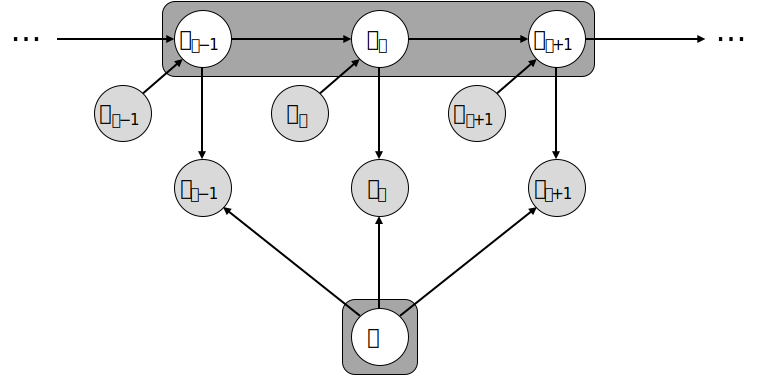
\includegraphics[keepaspectratio, scale=0.5]{figures/full-slam.pdf}
	\caption{完全SLAM問題の確率モデル}
	\label{fig:full-slam}
\end{figure}

\subsection{地図と計測の対応付け}
上記では地図$m$の具体的な表現については言及されなかった。ここでは例として、ロボットにレーザスキャナ(レーザレンジファインダ)を装着する場合を考える。このとき計測$z_t$はスキャンデータとよばれ、点群、即ち物体上の点までの距離$r$と方向$\theta$の集合として記述される。地図として点群(\textbf{特徴ベース}の地図)を用いるとき、スキャンデータ$z_t$に含まれる各点が、地図上のどの点と対応するのか判定する必要がある。このようなスキャンデータと地図との対応関係を、変数$c_t$として明示的に導入するのは有効である。また占有格子地図(\textbf{位置ベース}の地図)を用いるときも、スキャンデータ$z_t$を構成する各点と、地図上の格子との対応関係を考えることはできる。地図$m$と計測$z_t$との対応付け変数$c_t$を用いると、オンラインSLAM問題における事後確率は以下のようになる。
\begin{equation}
	p(x_t, m, c_t | z_{1 : t}, u_{1 : t})
\end{equation}
また完全SLAM問題の事後確率は次のように表される~\cite{Thrun07}\cite{Tomono16}\cite{Tomono18}。
\begin{equation}
	p(x_{1 : t}, m, c_{1 : t} | z_{1 : t}, u_{1 : t})
\end{equation}
オンラインSLAM問題での事後確率$p(x_t, m, c_t | z_{1 : t}, u_{1 : t})$は、完全SLAM問題での事後確率の周辺化として記述される。
\begin{equation}
	p(x_t, m, c_t | z_{1 : t}, u_{1 : t}) = \int \int \cdots \int \sum_{c_1} \sum_{c_2} \cdots \sum_{c_{t - 1}} p(x_{1 : t}, m, c_{1 : t} | z_{1 : t}, u_{1 : t}) dx_1 dx_2 \cdots dx_{t - 1}
\end{equation}
対応付け変数$c_t$が既知であれば、オンラインSLAM問題と完全SLAM問題における事後確率は、それぞれ次のようになる。先程とは異なり、計測確率の条件変数に$c_t$が加わって$p(z_t | x_t, m, c_t)$となる。
\begin{equation}
	p(x_t, m | z_{1 : t}, u_{1 : t}, c_{1 : t}) = \eta \ p(z_t | x_t, m, c_t) \int p(x_t | x_{t - 1}, u_t) p(x_{t - 1}, m | z_{1 : t - 1}, u_{1 : t - 1}, c_{1 : t - 1}) dx_{t - 1}
\end{equation}
\begin{eqnarray}
	p(x_{1 : t}, m | z_{1 : t}, u_{1 : t}, c_{1 : t}) &=& \eta \ p(z_t | x_t, m, c_t) p(x_t | x_{t - 1}, u_t) p(x_{1 : t - 1}, m | z_{1 : t - 1}, u_{1 : t - 1}, c_{1 : t - 1}) \\
	&=& \eta \ p(x_0, m) \prod_{t = 1}^t p(z_t | x_t, m, c_t) p(x_t | x_{t - 1}, u_t)
\end{eqnarray}
計測$z_t$には一般に複数個のデータが含まれるが、ここでは各データ$z_t^i$については互いに独立と仮定する。このとき計測確率は次のように、各データ$z_t^i$に関する項の積として記述できる。各データ$z_t^i$に割り振られる対応付け変数は$c_t^i$と表す。
\begin{equation}
	p(z_t | x_t, m, c_t) = \prod_i p(z_t^i | x_t, m, c_t^i)
\end{equation}
このとき完全SLAM問題は以下のように記述される。
\begin{equation}
	p(x_{1 : t}, m | z_{1 : t}, u_{1 : t}, c_{1 : t}) = \eta \ p(x_0, m) \prod_{t = 1}^t p(x_t | x_{t - 1}, u_t) \prod_i p(z_t^i | x_t, m, c_t^i)
\end{equation}

\subsection{完全SLAM問題の分解}
完全SLAM問題の事後確率は$p(x_{1 : t}, m, c_{1 : t} | z_{1 : t}, u_{1 : t})$であった。対応付け変数$c_{1 : t}$が既知、即ち計測$z_{1 : t}$と地図$m$との対応関係が完全に分かっているとき、完全SLAM問題は次の事後確率の推定となる。
\begin{equation}
	p(x_{1 : t}, m | z_{1 : t}, u_{1 : t}, c_{1 : t})
\end{equation}
地図$m$の構成要素を$\left\{ m_1, m_2, \ldots, m_N \right\}$と記述すると、上記の事後確率は次のように$N + 1$個の項に分解できる。各構成要素$m_n$は、点群地図(位置ベースの地図)であれば個々の点、占有格子地図(特徴ベースの地図)であれば単一の格子を意味する。軌跡$x_{1 : t}$が既知であれば、地図の各構成要素$m_n$は互いに独立になるため、地図$m$の推定は$N$個の各要素$m_n$の推定問題に分解できる。即ち完全SLAM問題は、対応関係$c_{1 : t}$が既知であれば、軌跡$x_{1 : t}$の推定と、地図の各構成要素$m_n$の推定という$N + 1$個の問題に分割される。これより、最初に軌跡$x_{1 : t}$のみを推定し、その軌跡を用いて地図の各要素$m_n$を個別に推定するという2段階の処理にできる。全時刻における状態$x_{1 : t}$と地図$m$を一度に推定しようとすると、途方もない計算が必要となる。地図$m$は大規模になる可能性があり、このとき解くべき問題は非常に高次元になる。高次元な空間に広がる確率分布$p(x_{1 : t}, m | z_{1 : t}, u_{1 : t}, c_{1 : t})$から、最大値を取るような解を探索するのは手間が掛かる。以下のように確率分布を$N + 1$個の項に分割すれば、各項を最大化する問題に置き換えられ、$x_{1 : t}$及び$m_n$の推定という低次元の問題に分割されるため、計算量を大幅に削減できる。
\begin{equation}
	p(x_{1 : t}, m | z_{1 : t}, u_{1 : t}, c_{1 : t}) = p(x_{1 : t} | z_{1 : t}, u_{1 : t}, c_{1 : t}) \prod_{n = 1}^N p(m_n | x_{1 : t}, z_{1 : t}, u_{1 : t}, c_{1 : t})
\end{equation}
上式の確率モデルは図\ref{fig:full-slam-with-associations}のように表現される。図\ref{fig:full-slam-with-associations}は、各時刻において計測データが一つであり、地図中のどれか一つの要素を観測する場合である。対応付け変数$c_t = j$が既知であることから、時刻$t$における計測$z_t$は、地図中の単一要素$m_j$に対するものだと分かる。時刻$t + 1$と$t + 2$では、対応付け変数$c_{t + 1}$と$c_{t + 2}$がいずれも$k$を指し示しており、従って同一の要素$m_k$が観測されている。ある時刻において複数の計測データが含まれ、地図中の複数の要素が同時に観測される場合は(複数の計測データが地図中の同一の要素を指すこともあり得る)、それと同じ個数分だけ対応付けの変数を用意すればよい。例えば各時刻において10個の計測データが得られるとき、その一つ一つが地図中のどの要素に対応するのかを示すために、各データについて10個の対応付け変数を導入すればよい。先程と同様に、計測データ$z_t = \left\{ z_t^i \right\}$について、各データ$z_t^i$に割り振られた対応付け変数を$c_t^i$と表す。\newline

図\ref{fig:full-slam-with-associations}に描かれた地図の各要素$m_i, \ m_j, \ m_k$をみると、いずれも状態変数$x_{t - 1}, \ x_t, \ x_{t + 1}, \ x_{t + 2}$を通じて間接的に接続されている。状態変数$x_{t - 1}, \ x_t, \ x_{t + 1}, \ x_{t + 2}$を通過することなく、地図中の2つの要素を結ぶようなパスは存在しないことから、全時刻における状態(軌跡)が既知であれば、地図中の各要素$m_i, \ m_j, \ m_k$は互いに独立になることが分かる。例えば、$m_j$の推定には軌跡$x_{1 : t}$、制御$u_{1 : t}$、計測$z_{1 : t}$、そして対応付け変数$c_{1 : t}$があれば十分であり、地図中の別の要素$m_i$は必要ではないため、要素$m_i$が正確に推定されても、$m_j$の推定には何ら影響を与えない。\newline

\begin{figure}[htbp]
	\centering
	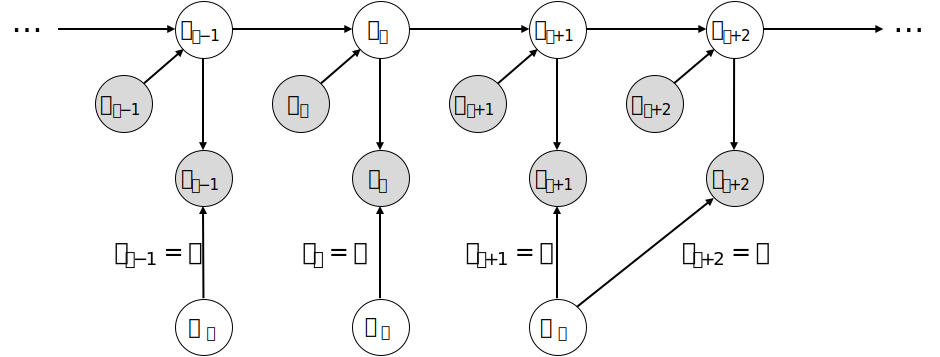
\includegraphics[keepaspectratio, scale=0.5]{figures/full-slam-with-associations.pdf}
	\caption{完全SLAM問題の分解}
	\label{fig:full-slam-with-associations}
\end{figure}

事後確率の分解を導出するために、まずは事後確率$p(x_{1 : t}, m | z_{1 : t}, u_{1 : t}, c_{1 : t})$を次のように分解する。この証明は文献~\cite{Thrun07}の13.2節を基にしている。
\begin{equation}
	p(x_{1 : t}, m | z_{1 : t}, u_{1 : t}, c_{1 : t}) = p(x_{1 : t} | z_{1 : t}, u_{1 : t}, c_{1 : t}) p(m | x_{1 : t}, z_{1 : t}, u_{1 : t}, c_{1 : t})
\end{equation}
第2項が、各要素$m_n$についての分布$p(m_n | x_{1 : t}, z_{1 : t}, u_{1 : t}, c_{1 : t})$の積として記述できることを、数学的帰納法によって示す。
\begin{equation}
	p(m | x_{1 : t}, z_{1 : t}, u_{1 : t}, c_{1 : t}) = \prod_{n = 1}^N p(m_n | x_{1 : t}, z_{1 : t}, u_{1 : t}, c_{1 : t})
\end{equation}
時刻$t = 0$のときは明らかに成立する。ロボットはまだ制御や計測を受け取っておらず、地図に関する知識を一切持たないため、地図の各要素$m_n$は互いに独立だからである。
\begin{equation}
	p(m) = \prod_{n = 1}^N p(m_n)
\end{equation}
時刻$t - 1$において上記の分解が成り立っているとき、時刻$t$についても成り立つことを示す。
\begin{equation}
	p(m | x_{1 : t - 1}, z_{1 : t - 1}, u_{1 : t - 1}, c_{1 : t - 1}) = \prod_{n = 1}^N p(m_n | x_{1 : t - 1}, z_{1 : t - 1}, u_{1 : t - 1}, c_{1 : t - 1})
\end{equation}
地図の各要素$m_n$について、時刻$t$で観測されたかどうかで場合分けを行う。観測されていれば、時刻$t$で得られた計測データ$z_t$の中には地図$m_n$に対応するものがあり($z_t^n$とする)、対応付け変数$c_t$には$n$が含まれている($c_t^n$とする)。時刻$t$で観測された要素の集合を$\mathcal{X}_t \subseteq \left\{ 1, \cdots, N \right\}$とすると、$\mathcal{X}_t$の各要素$n \in \mathcal{X}_t$について以下のようにできる。分母の第2項$p(m_n | x_{1 : t}, z_{1 : t - 1}, u_{1 : t}, c_{1 : t})$の変形では、時刻$t - 1$までの観測$z_{1 : t - 1}$が条件となっており、従って時刻$t$におけるロボットの状態$x_t$や制御$u_t$、対応付け変数$c_t$について独立となることを利用している。図\ref{fig:full-slam-with-associations}をみれば分かるように、時刻$t$で観測された地図の要素$m_n$は、時刻$t$における計測データ$z_t$と対応変数$c_t$を通じて状態$x_t$と関係しているため、時刻$t - 1$までの計測データ$z_{1 : t - 1}$の条件下では、$m_n$は対応変数$c_t$や状態$x_t$とは無関係になる。
\begin{eqnarray}
	p(m_n | x_{1 : t}, z_{1 : t}, u_{1 : t}, c_{1 : t}) &=& \frac{p(z_t^n | m_n, x_{1 : t}, z_{1 : t - 1}, u_{1 : t}, c_{1 : t}) p(m_n | x_{1 : t}, z_{1 : t - 1}, u_{1 : t}, c_{1 : t})}{p(z_t^n | x_{1 : t}, z_{1 : t - 1}, u_{1 : t}, c_{1 : t})} \\
	&=& \frac{p(z_t^n | m_n, x_t, c_t^n) p(m_n | x_{1 : t - 1}, z_{1 : t - 1}, u_{1 : t - 1}, c_{1 : t - 1})}{p(z_t^n | x_{1 : t}, z_{1 : t - 1}, u_{1 : t}, c_{1 : t})}
\end{eqnarray}
これより1時刻前までのデータによる$m_n$の事後確率について、次の式が得られる。
\begin{equation}
	p(m_n | x_{1 : t - 1}, z_{1 : t - 1}, u_{1 : t - 1}, c_{1 : t - 1}) = \frac{p(m_n | x_{1 : t}, z_{1 : t}, u_{1 : t}, c_{1 : t}) p(z_t^n | x_{1 : t}, z_{1 : t - 1}, u_{1 : t}, c_{1 : t})}{p(z_t^n | m_n, x_t, c_t^n)}
\end{equation}
地図の要素$m_n$が、時刻$t$で観測されていない場合を考える($m_n \notin \mathcal{X}_t$)。このとき$m_n$の事後確率は、1時刻前までのデータによって決まり、時刻$t$におけるロボットの状態$x_t$や制御$u_t$、対応付け変数$c_t$や計測$z_t$とは無関係になる。従って単に以下の式が成り立つ。
\begin{equation}
	p(m_n | x_{1 : t}, z_{1 : t}, u_{1 : t}, c_{1 : t}) = p(m_n | x_{1 : t - 1}, z_{1 : t - 1}, u_{1 : t - 1}, c_{1 : t - 1})
\end{equation}
上式の左辺と右辺を入れ替えれば以下のようになる。
\begin{equation}
	p(m_n | x_{1 : t - 1}, z_{1 : t - 1}, u_{1 : t - 1}, c_{1 : t - 1}) = p(m_n | x_{1 : t}, z_{1 : t}, u_{1 : t}, c_{1 : t})
\end{equation}
以上より$p(m_n | x_{1 : t - 1}, z_{1 : t - 1}, u_{1 : t - 1}, c_{1 : t - 1})$は、$m_n$が時刻$t$で観測されたかどうかによって、次のように場合分けできる。
\begin{eqnarray}
	p(m_n | x_{1 : t - 1}, z_{1 : t - 1}, u_{1 : t - 1}, c_{1 : t - 1}) &=& \left\{ \begin{array}{ll} \displaystyle \frac{p(m_n | x_{1 : t}, z_{1 : t}, u_{1 : t}, c_{1 : t}) p(z_t^n | x_{1 : t}, z_{1 : t - 1}, u_{1 : t}, c_{1 : t})}{p(z_t^n | m_n, x_t, c_t^n)} & (x \in \mathcal{X}_t) \\ p(m_n | x_{1 : t}, z_{1 : t}, u_{1 : t}, c_{1 : t}) & (x \notin \mathcal{X}_t) \end{array} \right.
\end{eqnarray}
これより、時刻$t$においても分解が成り立つことを示せる。
\begin{eqnarray}
	&& p(m | x_{1 : t}, z_{1 : t}, u_{1 : t}, c_{1 : t}) \nonumber \\
	&=& \frac{p(z_t | m, x_{1 : t}, z_{1 : t - 1}, u_{1 : t}, c_{1 : t}) p(m | x_{1 : t}, z_{1 : t - 1}, u_{1 : t}, c_{1 : t})}{p(z_t | x_{1 : t}, z_{1 : t - 1}, u_{1 : t}, c_{1 : t})} \qquad (\because ベイズの定理) \nonumber \\
	&=& \frac{p(z_t | m, x_t, c_t) p(m | x_{1 : t - 1}, z_{1 : t - 1}, u_{1 : t - 1}, c_{1 : t - 1})}{p(z_t | x_{1 : t}, z_{1 : t - 1}, u_{1 : t}, c_{1 : t})} \nonumber \\
	&=& \frac{p(z_t | m, x_t, c_t)}{p(z_t | x_{1 : t}, z_{1 : t - 1}, u_{1 : t}, c_{1 : t})} p(m | x_{1 : t - 1}, z_{1 : t - 1}, u_{1 : t - 1}, c_{1 : t - 1})
\end{eqnarray}
上式の第1項は、時刻$t$で観測された、地図の各要素$n \in \mathcal{X}_t$に関する項に分解できる。計測データに含まれる各計測については、互いに独立と仮定した。計測$z_t$に含まれる、各要素$n \in \mathcal{X}_t$に対応するものは$z_t^n$、そして対応付け変数は便宜的に$c_t^n$で表す。$n$は地図の各要素を指すインデックスであって、何番目の計測データかを表すインデックスではない。$c_t^n$は明らかに$n$を指している(前節での$z_t^i$と$c_t^i$の定義とは若干異なることに注意)。
\begin{equation}
	p(z_t | m, x_t, c_t) = \prod_{n \in \mathcal{X}_t} p(z_t^n | m_n, x_t, c_t^n)
\end{equation}
\begin{equation}
	p(z_t^n | x_{1 : t}, z_{1 : t - 1}, u_{1 : t}, c_{1 : t}) = \prod_{n \in \mathcal{X}_t} p(z_t^n | x_{1 : t}, z_{1 : t - 1}, u_{1 : t}, c_{1 : t})
\end{equation}
これを元の式に代入すれば次を得る。
\begin{eqnarray}
	&& p(m | x_{1 : t}, z_{1 : t}, u_{1 : t}, c_{1 : t}) \nonumber \\
	&=& \frac{\prod_{n \in \mathcal{X}_t} p(z_t^n | m_n, x_t, c_t^n)}{\prod_{n \in \mathcal{X}_t} p(z_t^n | x_{1 : t}, z_{1 : t - 1}, u_{1 : t}, c_{1 : t})} p(m | x_{1 : t - 1}, z_{1 : t - 1}, u_{1 : t - 1}, c_{1 : t - 1}) \nonumber \\
	&=& \frac{\prod_{n \in \mathcal{X}_t} p(z_t^n | m_n, x_t, c_t^n)}{\prod_{n \in \mathcal{X}_t} p(z_t^n | x_{1 : t}, z_{1 : t - 1}, u_{1 : t}, c_{1 : t})} \prod_{n = 1}^N p(m_n | x_{1 : t - 1}, z_{1 : t - 1}, u_{1 : t - 1}, c_{1 : t - 1}) \qquad (帰納法の仮定) \nonumber \\
	&=& \frac{\prod_{n \in \mathcal{X}_t} p(z_t^n | m_n, x_t, c_t^n)}{\prod_{n \in \mathcal{X}_t} p(z_t^n | x_{1 : t}, z_{1 : t - 1}, u_{1 : t}, c_{1 : t})} \nonumber \\
	&& \qquad \left[ \prod_{n \notin \mathcal{X}_t} p(m_n | x_{1 : t - 1}, z_{1 : t - 1}, u_{1 : t - 1}, c_{1 : t - 1}) \right] \left[ \prod_{n \in \mathcal{X}_t} p(m_n | x_{1 : t - 1}, z_{1 : t - 1}, u_{1 : t - 1}, c_{1 : t - 1}) \right] \nonumber
\end{eqnarray}
上記の$p(m_n | x_{1 : t - 1}, z_{1 : t - 1}, u_{1 : t - 1}, c_{1 : t - 1})$に、場合分けにより求めた式を代入すれば次を得る。
\begin{eqnarray}
	&& \frac{\prod_{n \in \mathcal{X}_t} p(z_t^n | m_n, x_t, c_t^n)}{\prod_{n \in \mathcal{X}_t} p(z_t^n | x_{1 : t}, z_{1 : t - 1}, u_{1 : t}, c_{1 : t})} \left[ \prod_{n \notin \mathcal{X}_t} p(m_n | x_{1 : t}, z_{1 : t}, u_{1 : t}, c_{1 : t}) \right] \nonumber \\
	&& \qquad \left[ \prod_{n \in \mathcal{X}_t} \frac{p(m_n | x_{1 : t}, z_{1 : t}, u_{1 : t}, c_{1 : t}) p(z_t^n | x_{1 : t}, z_{1 : t - 1}, u_{1 : t}, c_{1 : t})}{p(z_t^n | m_n, x_t, c_t^n)} \right] \nonumber \\
	&=& \frac{\prod_{n \in \mathcal{X}_t} p(z_t^n | m_n, x_t, c_t^n)}{\prod_{n \in \mathcal{X}_t} p(z_t^n | x_{1 : t}, z_{1 : t - 1}, u_{1 : t}, c_{1 : t})} \left[ \prod_{n \notin \mathcal{X}_t} p(m_n | x_{1 : t}, z_{1 : t}, u_{1 : t}, c_{1 : t}) \right] \nonumber \\
	&& \qquad \frac{\prod_{n \in \mathcal{X}_t} p(z_t^n | x_{1 : t}, z_{1 : t - 1}, u_{1 : t}, c_{1 : t})}{\prod_{n \in \mathcal{X}_t} p(z_t^n | m_n, x_t, c_t^n)} \left[ \prod_{n \in \mathcal{X}_t} p(m_n | x_{1 : t}, z_{1 : t}, u_{1 : t}, c_{1 : t}) \right] \nonumber
\end{eqnarray}
分母と分子が互いに打ち消し合うので、次のような単純な式になる。
\begin{eqnarray}
	&& \left[ \prod_{n \notin \mathcal{X}_t} p(m_n | x_{1 : t}, z_{1 : t}, u_{1 : t}, c_{1 : t}) \right] \left[ \prod_{n \in \mathcal{X}_t} p(m_n | x_{1 : t}, z_{1 : t}, u_{1 : t}, c_{1 : t}) \right] \nonumber \\
	&=& \prod_{n = 1}^N p(m_n | x_{1 : t}, z_{1 : t}, u_{1 : t}, c_{1 : t})
\end{eqnarray}
従って、対応関係$c_{1 : t}$が既知であるときの、完全SLAM問題の事後確率$p(x_{1 : t}, m | z_{1 : t}, u_{1 : t}, c_{1 : t})$は以下のように分解される~\cite{Thrun07}\cite{Tomono16}。
\begin{eqnarray}
	p(x_{1 : t}, m | z_{1 : t}, u_{1 : t}, c_{1 : t}) &=& p(x_{1 : t} | z_{1 : t}, u_{1 : t}, c_{1 : t}) p(m | x_{1 : t}, z_{1 : t}, u_{1 : t}, c_{1 : t}) \nonumber \\
	&=& p(x_{1 : t} | z_{1 : t}, u_{1 : t}, c_{1 : t}) \prod_{n = 1}^N p(m_n | x_{1 : t}, z_{1 : t}, u_{1 : t}, c_{1 : t})
\end{eqnarray}

\subsection{SLAM問題の難しさ}
SLAMでは、連続空間における姿勢$x_t$や地図$m$の推定(非線形最適化やフィルタ処理)だけでなく、離散的な対応付け変数$c_t$の推定、言い換えるとスキャンデータと地図の対応付け問題(組み合わせ最適化問題)を解く必要がある。このようにSLAMには連続的な問題と離散的な問題の双方が含まれている。連続的なパラメータ$x_t, m$、離散的なパラメータ$c_t$の個数は、普通どちらも大きくなる。非線形最適化により$x_t, m$を求める場合、次元数が大きくなると局所解に陥りやすくなる。また取り得る全ての対応付け$c_{1 : t}$の場合の数は、時刻$t$が大きくなるに従って指数的に増加する。これより解の候補は莫大になり、事後分布を厳密に求めることは不可能となる~\cite{Thrun07}\cite{Tomono16}\cite{Tomono18}。

\bibliographystyle{plain}
\bibliography{slam-formulation}

\end{document}
